\section{Differential Calculus}

\begin{Theorem}{
    Fundamental Lemma\footnote{\href{https://trello.com/c/byu9Pyy8}{Calculus with Analytic Geometry by George F. Simmons, 2nd}, p. 680}
    \phantomsection\hypertarget{fundamental-lemma}
}{fundamental-lemma}
    Suppose that a function $z = f(x, y)$ and its partial derivatives $f_x$ and $f_y$ are defined at a point
    $(x_0, y_0)$, and also through some neighborhood of this point. Suppose further that $f_x$ and $f_y$ are continuous
    at $(x_0, y_0)$. Then the increment $\Delta z$ can be expressed in the form of

    \begin{equation}
        \Delta z = f_x(x_0, y_0)\Delta x + f_y(x_0, y_0)\Delta y + \epsilon_1\Delta x + \epsilon_2\Delta y
    \end{equation}

    where $\epsilon_1$ and $\epsilon_2 \rightarrow 0$ as $\Delta x$ and $\Delta y \rightarrow 0$
\end{Theorem}

To prove this
statement\footnote{\href{https://trello.com/c/byu9Pyy8}{Calculus with Analytic Geometry by George F. Simmons, 2nd}, p. 841},
we analyze the change $\Delta z$ in 2 steps as shown in Fig.~\ref{fig:proof-fundamental-lemma}:

\begin{figure}[H]
    \centering
    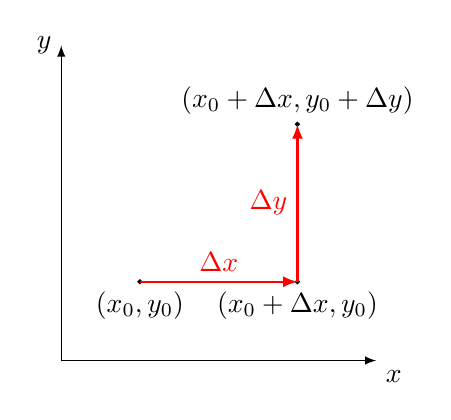
\begin{tikzpicture}
        \draw [<->] (0,4) -- (0,0) -- (4,0);
        \node [below right] at (4,0) {$x$};
        \node [left] at (0,4) {$y$};

        \draw[fill] (1,1) circle [radius=0.025];
        \draw[fill] (3,1) circle [radius=0.025];
        \draw[fill] (3,3) circle [radius=0.025];

        \node [below] at (1,1) {$(x_0, y_0)$};
        \node [below] at (3,1) {$(x_0 + \Delta x, y_0)$};
        \node [above] at (3,3) {$(x_0 + \Delta x, y_0 + \Delta y)$};

        \draw [->][thick, red] (1,1) -- node[above] {$\Delta x$} (3,1);
        \draw [->][thick, red] (3,1) -- node[left] {$\Delta y$} (3,3);
    \end{tikzpicture}
    \caption{We assume $\Delta z = f(x_0 + \Delta x, y_0 + \Delta y) - f(x_0, y_0)$ and $\Delta z = \Delta_1 z + \Delta_2 z$}
    \label{fig:proof-fundamental-lemma}
\end{figure}

\begin{enumerate}
    \item changing $x$ alone and moving from $(x_0, y_0)$ to $(x_0 + \Delta x, y_0)$, and then
    \item changing $y$ alone and moving from $(x_0 + \Delta x, y_0)$ to $(x_0 + \Delta x, y_0 + \Delta y)$
\end{enumerate}

We denote the first change in $z$ by $\Delta_1 z$, so that

\begin{equation}
    \Delta_1 z = f(x_0 + \Delta x, y_0) - f(x_0, y_0)
\end{equation}

By The Mean Value Theorem\footnote{
    \begin{Theorem}{
        The Mean Value Theorem\footnote{\href{https://trello.com/c/byu9Pyy8}{Calculus with Analytic Geometry by George F. Simmons, 2nd}, p. 76}
        \phantomsection\hypertarget{theo:mean-value-theorem}
    }{mean-value-theorem}
        Let $y = f(x)$ be a function with the following two properties:

        \begin{enumerate}
            \item $f(x)$ is continuous on the closed interval $[a, b]$; and
            \item $f(x)$ is differentiable on the open interval $(a, b)$
        \end{enumerate}

        Then there exists at least one point $c$ in the open interval $(a, b)$ such that

        \[
            f'(c) = \frac{f(b) - f(a)}{b - a}
        \]

        or equivalently,

        \[
            f(b) - f(a) = f'(c)(b - a)
        \]
    \end{Theorem}
}, we can write this as

\begin{equation}\label{eq:first-change-z-mean-val-theo}
\Delta_1 z = \Delta x f_x(x_1, y_0)
\end{equation}

where $x_1$ is between $x_0$ and $x_0 + \Delta x$. Smilary, if we denote the second part of the change in $z$ by
$\Delta_1 z$, so that

\begin{equation}
    \Delta_2 z = f(x_0 + \Delta x, y_0 + \Delta y) - f(x_0 + \Delta x, y_0)
\end{equation}

then

\begin{equation}\label{eq:second-change-z-mean-val-theo}
\Delta_2 z = \Delta y f_y(x_0 + \Delta x, y_1)
\end{equation}

where $y_1$ is between $y_0$ and $y_0 + \Delta y$.

Now as $\Delta x$ and $\Delta y \rightarrow 0$, $x_1 \rightarrow x_0$ and $y_1 \rightarrow y_0$. By the assumed
continuity of $f_x$ and $f_y$ at $(x_0, y_0)$, we can write

\begin{align}
    f_x(x_1, y_0) = f_x(x_0, y_0) + \epsilon_1 \label{eq:first-change-z-epsilon} \\
    f_y(x_0 + \Delta x, y_1) = f_y(x_0, y_0) + \epsilon_2 \label{eq:second-change-z-epsilon}
\end{align}

where $\epsilon_1$ and $\epsilon_2 \rightarrow 0$ as $\Delta x$ and $\Delta y \rightarrow 0$. Plugging
Eq.\ref{eq:first-change-z-epsilon} into Eq.\ref{eq:first-change-z-mean-val-theo} gives us

\begin{equation}
    \Delta_1 z = \Delta x\left[ f_x(x_0, y_0) + \epsilon_1 \right] = \Delta x f_x(x_0, y_0) + \Delta x\epsilon_1
\end{equation}

and similarly Eq.\ref{eq:second-change-z-epsilon} into Eq.\ref{eq:second-change-z-mean-val-theo}

\begin{equation}
    \Delta_2 z = \Delta y\left[ f_y(x_0, y_0) + \epsilon_2 \right] = \Delta y f_y(x_0, y_0) + \Delta y\epsilon_2
\end{equation}

Since we have assumed $\Delta z = \Delta_1 z + \Delta_2 z$

\begin{equation}
    \Delta z = \Delta x f_x(x_0, y_0) + \Delta x\epsilon_1 + \Delta y f_y(x_0, y_0) + \Delta y\epsilon_2 = f_x(x_0, y_0)\Delta x + f_y(x_0, y_0)\Delta y + \epsilon_1\Delta x + \epsilon_2\Delta y
\end{equation}

\begin{figure}[H]
    \begin{flushright}
        
\includegraphics[width=0.05\textwidth]{胡桃-28.png}
    \end{flushright}
\end{figure}

\footnote{\href{https://trello.com/c/byu9Pyy8}{Calculus with Analytic Geometry by George F. Simmons, 2nd}, p. 681} Now Let
$f(x, y, z)$ be a function of 3 variables defined throughout some region of three-dimensional space, and let $P$ be a
point in this region. At what rate does $f$ change as we move away from $P$ in a specified direction? In the directions
of the positive x, y, and z-axes, we know that the rates of change off are given by the partial derivatives
$\frac{\partial f}{\partial x}$, $\frac{\partial f}{\partial y}$, and $\frac{\partial f}{\partial z}$. But how do we
calculate the rate of change of $f$ if we move away from $P$ in a direction that is not a coordinate direction?

Let $P = (x, y, z)$ and $\boldsymbol{R} = x\boldsymbol{i} + y\boldsymbol{j} + z\boldsymbol{k}$ being the position vector
of $P$. If we move away from $P$ to a nearby point $Q = (x + \Delta x, y + \Delta y, z + \Delta z)$, then the function
will change by an amoutn $\Delta f$. Let $\Delta s$ denote the distance between $P$ and $Q$, then we have

\begin{equation}\label{eq:def-df-over-ds}
    \frac{df}{ds} = \lim\limits_{\Delta s \rightarrow 0}\frac{\Delta f}{\Delta s}
\end{equation}

We further assume that $f(x, y, z)$ has continuous partial derivatives with respect to $x$, $y$, and $z$.

\begin{marker}
    Unless explicitly stated otherwise, all functions we deal with are always continuous in all of our discussions
\end{marker}

The \hyperlink{fundamental-lemma}{Fundamental Lemma} enables us to write $\Delta f$ in the form of

\begin{equation}\label{eq:df-in-3-partials}
    \Delta f = \frac{\partial f}{\partial x}\Delta x + \frac{\partial f}{\partial y}\Delta y + \frac{\partial f}{\partial z}\Delta z + \epsilon_1\Delta x + \epsilon_2\Delta y + \epsilon_3\Delta z
\end{equation}

As $\Delta s \rightarrow 0$, i.e. as $\Delta x \rightarrow 0$, $\Delta y \rightarrow 0$, and $\Delta z \rightarrow 0$,
$\epsilon_1, \epsilon_2, \epsilon_3 \rightarrow 0$. Dividing Eq.\ref{eq:df-in-3-partials} by $\Delta s$ gives

\begin{equation}\label{eq:df-over-ds-in-3-partials}
    \lim\limits_{\Delta s \rightarrow 0}\frac{\Delta f}{\Delta s} = \frac{\partial f}{\partial x}\frac{dx}{ds} + \frac{\partial f}{\partial y}\frac{dy}{ds} + \frac{\partial f}{\partial z}\frac{dz}{ds}
\end{equation}

Combing Eq.\ref{eq:df-over-ds-in-3-partials} and \ref{eq:def-df-over-ds} results in

\begin{equation}\label{eq:partial-chain-rule}
    \tcbhighmath[
        enhanced,colframe=red,colback=white,arc=0pt,boxrule=1pt,
        fuzzy halo=1mm with blue!50!white,
        arc=2pt,
        boxrule=0pt,
        frame hidden
    ]{
        \frac{df}{ds} = \frac{\partial f}{\partial x}\frac{dx}{ds} + \frac{\partial f}{\partial y}\frac{dy}{ds} + \frac{\partial f}{\partial z}\frac{dz}{ds}
    }
\end{equation}

\subsection{Gradient}

\footnote{\href{https://trello.com/c/U6HhhDq6}{Introduction to Electrodynamics by Griffiths, 3rd}, p. 13} The theorem
on \hyperref[eq:partial-chain-rule]{partial derivaves states} that

\begin{equation}
    dT = \left( \frac{\partial T}{\partial x} \right) dx + \left( \frac{\partial T}{\partial y} \right) dy + \left( \frac{\partial T}{\partial z} \right) dz
\end{equation}

Writing it in the dot product form:

\begin{align}
    dT &= \left( \frac{\partial T}{\partial x}\boldsymbol{\hat{x}} + \frac{\partial T}{\partial y}\boldsymbol{\hat{y}} + \frac{\partial T}{\partial z}\boldsymbol{\hat{z}} \right) \cdot (dx\boldsymbol{\hat{x}} + dy\boldsymbol{\hat{y}} + dz\boldsymbol{\hat{z}}) \\
      &= \nabla T \cdot d\boldsymbol{l} \label{eq:dt-dot}
\end{align}

where

\begin{equation}\label{eq:def-gradient}
    \nabla T \equiv \frac{\partial T}{\partial x}\boldsymbol{\hat{x}} + \frac{\partial T}{\partial y}\boldsymbol{\hat{y}} + \frac{\partial T}{\partial z}\boldsymbol{\hat{z}}
\end{equation}

is the \textbf{gradient} of $T$. We also call $\nabla$ as the \textbf{vector operator} that \textit{acts upon} $T$

\begin{tcolorbox}[
    parbox=false,
    colbacktitle=red!10!white,
    colback=blue!10!white,coltitle=red!70!black,
    title=The Geometrical Interpretation of the Gradient
]
    The doc product~\ref{eq:dt-dot} can be written as

    \begin{equation}
        dT = \nabla T \cdot d\boldsymbol{l} = \vert \nabla T \vert \vert d\boldsymbol{l} \vert \cos{\theta}
    \end{equation}

    We soon realize that the \textit{maximum} change of T occurs when $\theta = 0$, therefore

    \begin{tcolorbox}[colback=red!10!white]
        \begin{center}
            \textcolor[HTML]{8F8FF5}{\textbf{The gradient $\nabla T$ points in the direction of the maximum increase of $T$,
            and its magnitude $\vert \nabla T \vert$ gives the slope (rate of increase) along this maximal direction}}
        \end{center}
    \end{tcolorbox}
\end{tcolorbox}

Now there are 3 ways the operator $\nabla$ can act:

\begin{enumerate}
    \item On a scalar function $T$: $\nabla T$ (the gradient, which we've discussed so far)
    \item On a vector function via the dot product: $\nabla \cdot \boldsymbol{v}$ (the \textbf{divergence})
    \item On a vector function via the cross product: $\nabla \times \boldsymbol{v}$ (the \textbf{curl})
\end{enumerate}

\subsection{Divergence}

From \hyperref[eq:def-gradient]{the definition of $\nabla$}, we construct the divergence

\begin{align}
    \nabla \cdot \boldsymbol{v} &= \left( \frac{\partial T}{\partial x}\boldsymbol{\hat{x}} + \frac{\partial T}{\partial y}\boldsymbol{\hat{y}} + \frac{\partial T}{\partial z}\boldsymbol{\hat{z}} \right) \cdot (v_x\boldsymbol{\hat{x}} + v_y\boldsymbol{\hat{y}} + v_z\boldsymbol{\hat{z}}) \label{eq:divergence-dot-product} \\
    &= \frac{\partial v_x}{\partial x} + \frac{\partial v_y}{\partial y} + \frac{\partial v_z}{\partial z}
\end{align}

\subsubsection{The Meaning of Divergence}

\begin{tcolorbox}[
    parbox=false,
    colbacktitle=red!10!white,
    colback=blue!10!white,coltitle=red!70!black,
    title=The Geometrical Interpretation of the Divergence
]
    The divergence is a measure of how much the vector $\boldsymbol{v}$ spreads out (diverges) from the point in question
\end{tcolorbox}

\begin{figure}[H]
    \tikzset{>=latex}
    \colorlet{veccol}{orange!90!black}
    \colorlet{myblue}{blue!60!black}
    \tikzstyle{vector}=[->,thick,veccol]
    \def\R{1.4}
    \def\r{0.03}
    \def\N{9}
    \def\null{\color{myblue}{0}}
    \centering
    \begin{subfigure}{.24\textwidth}
        \centering
        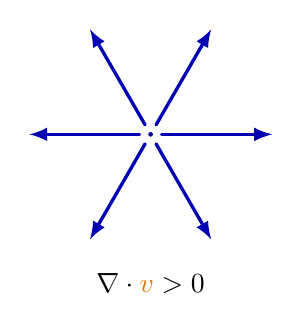
\begin{tikzpicture}
            \fill[myblue] (0,0) circle (\r);
            \foreach \i [evaluate={\ang=\i*360/\N;}] in {0,...,\N}{
                \draw[vector] (\ang:0.1*\R) --++ (\ang:\R);
            }
            \node at (0,-1.35*\R) {$\nabla \cdot {{\color{veccol}\boldsymbol{v}}} > 0$};
        \end{tikzpicture}
    \end{subfigure}
    \begin{subfigure}{.24\textwidth}
        \centering
        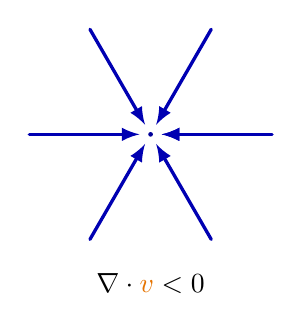
\begin{tikzpicture}
            \fill[myblue] (0,0) circle (\r);
            \foreach \i [evaluate={\ang=\i*360/\N;}] in {0,...,\N}{
                \draw[vector] (\ang:1.1*\R) -- (\ang:0.1*\R);
            }
            \node at (0,-1.35*\R) {$\nabla \cdot {{\color{veccol}\boldsymbol{v}}} < 0$};
        \end{tikzpicture}
    \end{subfigure}
    \begin{subfigure}{.24\textwidth}
        \centering
        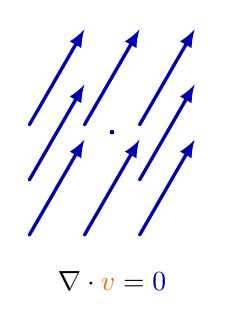
\begin{tikzpicture}
            \def\ang{60}
            \fill[myblue] (0,0) circle (\r);
            \foreach \x/\y in {-1/0,-1/1,0/1,1/1,1/0,-1/-1,0/-1,1/-1}{
                \draw[vector] (\x*0.5*\R,\y*0.5*\R) ++ (\ang-180:\R/2) --++ (\ang:\R);
            }
            \node at (0,-1.35*\R) {$\nabla \cdot {{\color{veccol}\boldsymbol{v}}} = \null$};
        \end{tikzpicture}
    \end{subfigure}
    \begin{subfigure}{.24\textwidth}
        \centering
        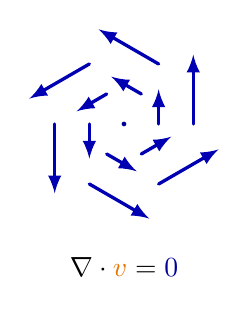
\begin{tikzpicture}
            \def\ang{60}
            \def\N{6}
            \fill[myblue] (0,0) circle (\r);
            \foreach \R in {0.44,0.88}{
                \foreach \i [evaluate={\ang=\i*360/\N;}] in {1,...,\N}{
                    \draw[vector] (\ang:\R) --++ (\ang+90:\R);
                }
            }
            \node at (0,-1.3*\R) {$\nabla \cdot {{\color{veccol}\boldsymbol{v}}} = \null$};
        \end{tikzpicture}
    \end{subfigure}
    \caption{Divergence of vector fields}
    \label{fig:divergence-examples}
\end{figure}

\subsection{Curl}

\subsubsection{The Cross Prudct of Two Vectors}

\footnote{\href{https://trello.com/c/byu9Pyy8}{Calculus with Analytic Geometry by George F. Simmons, 2nd}, p. 640} Many
problems in geometry require us to find a vector that is perpendicular to each of two given vectors $\boldsymbol{A}$ and
$\boldsymbol{B}$. A routine way of doing this is provided by the \textit{cross product} (or \textit{vector product}) of
$\boldsymbol{A}$ and $\boldsymbol{B}$, denoted by $\boldsymbol{A} \times \boldsymbol{B}$. This cross product is very
different from the \hyperref[eq:divergence-dot-product]{dot product} $\boldsymbol{A} \cdot \boldsymbol{B}$, because
$\boldsymbol{A} \times \boldsymbol{B}$ is a vector while $\boldsymbol{A} \cdot \boldsymbol{B}$ is a scalar.

Consider two nonzero vectors $\boldsymbol{A}$ and $\boldsymbol{B}$. Suppose their tails conincide and let $\theta$ be
the angle from $\boldsymbol{A}$ to $\boldsymbol{B}$ (\textit{not} from $\boldsymbol{B}$ to $\boldsymbol{A}$) with
$0 \le \theta \le \pi$.

\begin{figure}[H]
    \centering
    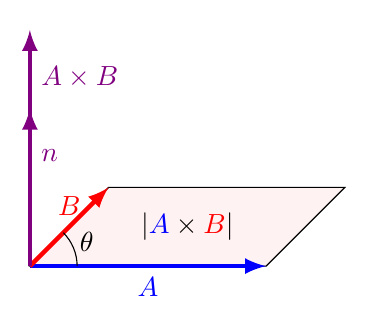
\begin{tikzpicture}
        \draw[-,fill=white!95!red](0,0)--(3,0)--(4,1)--(1,1)--cycle;
        \node at (2,0.5) {$|\textcolor{blue}{\boldsymbol{A}}\times \textcolor{red}{\boldsymbol{B}}|$};
        \draw[ultra thick,-latex,blue](0,0)--(3,0)node[midway,below]{$\boldsymbol{A}$};
        \draw[ultra thick,-latex,red](0,0)--(1,1)node[midway,above]{$\boldsymbol{B}$};
        \draw[ultra thick,-latex,blue!50!red](0,0)--(0,3)node[pos=0.8,right]{$\boldsymbol{A} \times \boldsymbol{B}$};
        \draw[ultra thick,-latex,blue!50!red](0,0)--(0,2)node[pos=0.7,right]{$\boldsymbol{n}$};
        \draw (0.6,0) arc [start angle=0,end angle=45,radius=0.6]
        node[pos=0.7,right]{$\theta$};
    \end{tikzpicture}
    \caption{The plane defined by $\boldsymbol{A}$ and $\boldsymbol{B}$}
    \label{fig:cross-prod}
\end{figure}

These 2 vectors determine a plane, as shown in Fig.~\ref{fig:cross-prod}. We now choose the unit
vector $\boldsymbol{n}$ which is normal (perpendicular) to this plane and whose direction is determined by the
\textit{right-hand thumb rule}\footnote{This means that if the right hand is placed so that the thumb is perpendicular
to the plane of $\boldsymbol{A}$ and $\boldsymbol{B}$ and the fingers curl from $\boldsymbol{A}$ to $\boldsymbol{B}$ in
the direction of angle $\theta$, then $\boldsymbol{n}$ points in the same direction as the thumb of this hand}.
\textit{This gives the direction of $\boldsymbol{A} \times \boldsymbol{B}$}

Vectors $\boldsymbol{A}$ and $\boldsymbol{B}$ also defines a parallelogram in this plane of area
$\vert \boldsymbol{A} \vert\vert \boldsymbol{B} \vert\sin{\theta}$, which defines \textit{the magnitude of
$\boldsymbol{A} \times \boldsymbol{B}$}.

\begin{Definition}{Cross Product of $\boldsymbol{A}$ and $\boldsymbol{B}$}{cross-product}
    \begin{equation}
        \boldsymbol{A} \times \boldsymbol{B} = \vert \boldsymbol{A} \vert\vert \boldsymbol{B} \vert\sin{\theta}
    \end{equation}
\end{Definition}

Our next objective is to develop a convenient formula for calculating $\boldsymbol{A} \times \boldsymbol{B}$ where

\begin{equation}\label{eq:cross-product-of-two}
    \boldsymbol{A} = a_1\boldsymbol{\hat{i}} + a_2\boldsymbol{\hat{j}} + a_3\boldsymbol{\hat{k}} \text{\ \ \ \ \ \ and \ \ \ \ \ \ }
    \boldsymbol{B} = b_1\boldsymbol{\hat{i}} + b_2\boldsymbol{\hat{j}} + b_3\boldsymbol{\hat{k}}
\end{equation}

We need to know that the cross product possesses the following algebraic properties

\begin{align}
    (c\boldsymbol{A}) \times \boldsymbol{B} &= c(\boldsymbol{A} \times \boldsymbol{B}) = \boldsymbol{A} \times (c\boldsymbol{B})\label{eq:cross-product-homogeneity}, \\
    \boldsymbol{A} \times (\boldsymbol{B} + \boldsymbol{C}) &= \boldsymbol{A} \times \boldsymbol{B} + \boldsymbol{A} \times \boldsymbol{C}\label{eq:cross-product-distributive-right}, \\
    (\boldsymbol{A} + \boldsymbol{B}) \times \boldsymbol{C} &= \boldsymbol{A} \times \boldsymbol{C} + \boldsymbol{B} \times \boldsymbol{C}\label{eq:cross-product-distributive-left}
\end{align}

Property~\ref{eq:cross-product-homogeneity}, also called \textit{homogeneous} in each
argument\footnote{\href{https://en.wikiversity.org/wiki/Cross_product}{Cross product}, Wikiversity}, is easily
established directly from Definition~\ref{def:cross-product}.

The proof of Eq.~\ref{eq:cross-product-distributive-right} starts with a unit vector $\boldsymbol{\hat{n}}$ and 3
arbitrary vectors $\boldsymbol{B}$, $\boldsymbol{C}$, and $\boldsymbol{B + C}$.
$\boldsymbol{\hat{n}} \times \boldsymbol{(B + C)}$ can be constructed by performing the following two operations:

\begin{figure}[H]
    \centering
    \begin{tikzpicture}[x=1cm, y=1cm, z=-0.6cm]
        \fill[white!95!red](-3, 0, 2.5)--(3, 0, 2.5)--(3.5, 0, -1)--(-2.5, 0, -1)--cycle;

        % Axes
        \draw [thick, -{latex[scale=3.0]}] (0,0,0) -- (0,1,0) node [at end, right] {$\boldsymbol{A}$};

        % Vectors
        \draw [very thick, -{latex[scale=3.0]}, white!45!red] (0,0,0) -- (-1,3,1)node[pos=0.7,right]{$\boldsymbol{B} + \boldsymbol{C}$};
        \draw [very thick, -{latex[scale=3.0]}, white!45!red] (0,0,0) -- (0,2,2)node[pos=0.5,below]{$\boldsymbol{B}$};
        \draw [very thick, -{latex[scale=3.0]}, white!45!red] (0,2,2) -- (-1,3,1)node[pos=0.5,left]{$\boldsymbol{C}$};

        \draw [very thick, -{latex[scale=3.0]}, white!45!red] (0,0,0) -- (-1,0,1)node[pos=1.0,above]{$(\boldsymbol{B} + \boldsymbol{C})'$};
        \draw [very thick, -{latex[scale=3.0]}, white!45!red] (0,0,0) -- (0,0,2)node[pos=0.9,below]{$\boldsymbol{B}'$};
        \draw [very thick, -{latex[scale=3.0]}, white!45!red] (0,0,2) -- (-1,0,1)node[pos=0.4,left]{$\boldsymbol{C}'$};

        \draw [very thick, -{latex[scale=3.0]}, white!45!red] (0,0,0) -- (1,0,1)node[pos=0.9,below]{$(\boldsymbol{B} + \boldsymbol{C})''$};
        \draw [very thick, -{latex[scale=3.0]}, white!45!red] (0,0,0) -- (2,0,0)node[pos=1.0,above]{$\boldsymbol{B}''$};
        \draw [very thick, -{latex[scale=3.0]}, white!45!red] (2,0,0) -- (1,0,1)node[pos=0.6,below]{$\boldsymbol{C}''$};

        % Dashes
        \draw [loosely dashed, thick] (-1,3,1) -- (-1,0,1);
        \draw [loosely dashed, thick] (0,2,2) -- (0,0,2);

        \draw [line width=0mm, white!45!red] (0, 0, 1) coordinate (a)
        -- (0, 0, 0) coordinate (b)
        -- (1, 0, 0) coordinate (c)
        pic["$\theta$", draw=black, <->, angle eccentricity=1.5, angle radius=0.3cm] {angle=a--b--c};
    \end{tikzpicture}
\end{figure}

\begin{enumerate}
    \item Project $\boldsymbol{B}$, $\boldsymbol{C}$, and $\boldsymbol{(B + C)}$ onto the plane perpendicular to
          $\boldsymbol{\hat{n}}$ to obtain a vector $\boldsymbol{B}'$, $\boldsymbol{C}'$, and $\boldsymbol{(B + C)'}$.
          By the nature of projection, the head and tails of $\boldsymbol{B'}$, $\boldsymbol{C'}$, and
          $\boldsymbol{(B + C)'}$ still coincide. Then,
    \item rotate the triangle formed by $\boldsymbol{B}'$, $\boldsymbol{C}'$, and $\boldsymbol{(B + C)'}$ by 90 degrees
          counterclockwise with respect to the tail of $\boldsymbol{\hat{n}}$ to obtain $\boldsymbol{B}''$,
          $\boldsymbol{C}''$, and $\boldsymbol{(B + C)''}$, which still form a triangle.
\end{enumerate}

Therefore, we have

\[
    (\boldsymbol{B} + \boldsymbol{C})'' = \boldsymbol{B}'' + \boldsymbol{C}''
\]

What this means is, geometrically, the operation of $\boldsymbol{\hat{n}} \times (\boldsymbol{B} + \boldsymbol{C})$ and
$\boldsymbol{\hat{n}} \times \boldsymbol{B} + \boldsymbol{\hat{n}} \times \boldsymbol{C}$ produces the same result, i.e.
the vector $(\boldsymbol{B} + \boldsymbol{C})''$. Therefore

\[
    \boldsymbol{\hat{n}} \times (\boldsymbol{B} + \boldsymbol{C}) = \boldsymbol{\hat{n}} \times \boldsymbol{B} + \boldsymbol{\hat{n}} \times \boldsymbol{C}
\]

Now let

\begin{equation}
    \boldsymbol{A} = c \boldsymbol{\hat{n}}
\end{equation}

We will then have

\[
    \cancel{\frac{1}{c}}\boldsymbol{A} \times (\boldsymbol{B} + \boldsymbol{C}) = \cancel{\frac{1}{c}}\boldsymbol{A} \times \boldsymbol{B} + \cancel{\frac{1}{c}}\boldsymbol{A} \times \boldsymbol{C}
\]

ending up with the original formula of

\[
    \boldsymbol{A} \times (\boldsymbol{B} + \boldsymbol{C}) = \boldsymbol{A} \times \boldsymbol{B} + \boldsymbol{A} \times \boldsymbol{C}
\]

\begin{figure}[H]
    \begin{flushright}
        
\includegraphics[width=0.05\textwidth]{胡桃-28.png}
    \end{flushright}
\end{figure}

Eq.~\ref{eq:cross-product-distributive-left} follows from Eq~\ref{eq:cross-product-distributive-right} combined with the
corollary of

\begin{equation}
    \boldsymbol{A} \times \boldsymbol{B} = - \boldsymbol{B} \times \boldsymbol{A}
\end{equation}

\begin{align*}
    (\boldsymbol{A} + \boldsymbol{B}) \times \boldsymbol{C} &= - \left[ \boldsymbol{C} \times (\boldsymbol{A} + \boldsymbol{B}) \right] \\
    &= - (\boldsymbol{C} \times \boldsymbol{A} + \boldsymbol{C} \times \boldsymbol{B}) \\
    &= - \boldsymbol{C} \times \boldsymbol{A} - \boldsymbol{C} \times \boldsymbol{B} \\
    &= \boldsymbol{A} \times \boldsymbol{C} + \boldsymbol{B} \times \boldsymbol{C}
\end{align*}

\begin{figure}[H]
    \begin{flushright}
        
\includegraphics[width=0.05\textwidth]{胡桃-28.png}
    \end{flushright}
\end{figure}

We continue with our task of multiplying out the \hyperref[eq:cross-product-of-two]{cross product of the vectors} using
Eq.~\ref{eq:cross-product-homogeneity},~\ref{eq:cross-product-distributive-right}, and ~\ref{eq:cross-product-distributive-left}.
By substituting $b_1\boldsymbol{\hat{i}} + b_2\boldsymbol{\hat{j}} + b_3\boldsymbol{\hat{k}}$ with $\boldsymbol{B}$:

\begin{align}
    \boldsymbol{A} \times \boldsymbol{B} &= (a_1\boldsymbol{\hat{i}} + a_2\boldsymbol{\hat{j}} + a_3\boldsymbol{\hat{k}}) \times (b_1\boldsymbol{\hat{i}} + b_2\boldsymbol{\hat{j}} + b_3\boldsymbol{\hat{k}}) \\
    &= (a_1\boldsymbol{\hat{i}} + a_2\boldsymbol{\hat{j}} + a_3\boldsymbol{\hat{k}}) \times \boldsymbol{B}\label{eq:cross-product-assumed-distributivity} \\
    &= a_1\boldsymbol{\hat{i}} \times \boldsymbol{B} + a_2\boldsymbol{\hat{j}} \times \boldsymbol{B} + a_3\boldsymbol{\hat{k}} \times \boldsymbol{B} \\
    &= a_1\boldsymbol{\hat{i}} \times (b_1\boldsymbol{\hat{i}} + b_2\boldsymbol{\hat{j}} + b_3\boldsymbol{\hat{k}}) + a_2\boldsymbol{\hat{j}} \times (b_1\boldsymbol{\hat{i}} + b_2\boldsymbol{\hat{j}} + b_3\boldsymbol{\hat{k}}) + a_3\boldsymbol{\hat{k}} \times (b_1\boldsymbol{\hat{i}} + b_2\boldsymbol{\hat{j}} + b_3\boldsymbol{\hat{k}}) \\
    &= a_1 b_1 \boldsymbol{\hat{i}} \times \boldsymbol{\hat{i}} + a_1 b_2 \boldsymbol{\hat{i}} \times \boldsymbol{\hat{j}} + a_1 b_3 \boldsymbol{\hat{i}} \times \boldsymbol{\hat{k}} + a_2 b_1 \boldsymbol{\hat{j}} \times \boldsymbol{\hat{i}} + a_2 b_2 \boldsymbol{\hat{j}} \times \boldsymbol{\hat{j}} + a_2 b_3 \boldsymbol{\hat{j}} \times \boldsymbol{\hat{k}} + a_3 b_1 \boldsymbol{\hat{k}} \times \boldsymbol{\hat{i}} + a_3 b_2 \boldsymbol{\hat{k}} \times \boldsymbol{\hat{j}} + a_3 b_3 \boldsymbol{\hat{k}} \times \boldsymbol{\hat{k}}\label{eq:cross-product-complete-expand}
\end{align}

With the following corollaries,

\begin{align}
    \boldsymbol{\hat{i}} \times \boldsymbol{\hat{i}} = 0 \\
    \boldsymbol{\hat{j}} \times \boldsymbol{\hat{j}} = 0 \\
    \boldsymbol{\hat{k}} \times \boldsymbol{\hat{k}} = 0 \\
    \boldsymbol{\hat{i}} \times \boldsymbol{\hat{j}} = -\boldsymbol{\hat{j}} \times \boldsymbol{\hat{i}} = \boldsymbol{\hat{k}} \\
    \boldsymbol{\hat{j}} \times \boldsymbol{\hat{k}} = -\boldsymbol{\hat{k}} \times \boldsymbol{\hat{j}} = \boldsymbol{\hat{i}} \\
    \boldsymbol{\hat{k}} \times \boldsymbol{\hat{i}} = -\boldsymbol{\hat{i}} \times \boldsymbol{\hat{k}} = \boldsymbol{\hat{j}} \\
\end{align}

Eq.~\ref{eq:cross-product-complete-expand} simplifies down to

\begin{align}
    \boldsymbol{A} \times \boldsymbol{B} &= a_1 b_2 \boldsymbol{\hat{k}} - a_1 b_3 \boldsymbol{\hat{j}} - a_2 b_1 \boldsymbol{\hat{k}} + a_2 b_3 \boldsymbol{\hat{i}} + a_3 b_1 \boldsymbol{\hat{j}} - a_3 b_2 \boldsymbol{\hat{i}} \\
    &= (a_2 b_3 - a_3 b_2)\boldsymbol{\hat{i}} - (a_1 b_3 - a_3 b_1)\boldsymbol{\hat{j}} + (a_1 b_2 - a_2 b_1)\boldsymbol{\hat{k}}\label{eq:cross-product-algebraic-expand}
\end{align}

We recall that a determinant of order 2 is defined by

\begin{equation}
    \begin{vmatrix}
        a_1 & a_2 \\
        b_1 & b_2 \\
    \end{vmatrix} = a_1 b_2 - a_2 b_1
\end{equation}

A determinant of order 3 can be defined in terms of determinants of order 2 as

\begin{equation}
    \begin{vmatrix}
        a_1 & a_2 & a_3 \\
        b_1 & b_2 & b_3 \\
        c_1 & c_2 & c_3 \\
    \end{vmatrix} =
    a_1 \begin{vmatrix}
        b_2 & b_3 \\
        c_2 & c_3 \\
    \end{vmatrix} -
    a_2 \begin{vmatrix}
        b_1 & b_3 \\
        c_1 & c_3 \\
    \end{vmatrix} +
    a_3 \begin{vmatrix}
        b_1 & b_2 \\
        c_1 & c_2 \\
    \end{vmatrix}
\end{equation}

Eq.~\ref{eq:cross-product-algebraic-expand} is equivalent to

\begin{align}
    \boldsymbol{A} \times \boldsymbol{B} &=
    \begin{vmatrix}
        a_2 & a_3 \\
        b_2 & b_3 \\
    \end{vmatrix} \boldsymbol{\hat{i}} -
    \begin{vmatrix}
        a_1 & a_3 \\
        b_1 & b_3 \\
    \end{vmatrix} \boldsymbol{\hat{j}} +
    \begin{vmatrix}
        a_1 & a_2 \\
        b_1 & b_2 \\
    \end{vmatrix} \boldsymbol{\hat{k}} \\ &=
    \begin{vmatrix}
        \boldsymbol{\hat{i}} & \boldsymbol{\hat{j}} & \boldsymbol{\hat{j}} \\
        a_1 & a_2 & a_3 \\
        b_1 & b_2 & b_3 \\
    \end{vmatrix} \label{eq:cross-product-algebraic-form}
\end{align}

\begin{tcolorbox}[
    parbox=false,
    enhanced,
    colback=red!5!white,colframe=red!75!black,
    watermark tikz={\draw[line width=2mm] circle (1cm) node{\fontfamily{ptm}\fontseries{b}\fontsize{20mm}{20mm}\selectfont !};}
]
    It should be noted that formula~\ref{eq:cross-product-algebraic-form} is by no means a definition of cross product,
    because obtaining it must assume the \hyperref[eq:cross-product-assumed-distributivity]{distributivity law}
    \footnote{\href{https://math.stackexchange.com/questions/362139/how-to-prove-the-distributive-property-of-cross-product\#comment5670827\_362161}{The determinant pre-assumes the distributivity of cross product}}.
    We should view \ref{eq:cross-product-algebraic-form} simply as a convenient tool for making calculations

    In addition, Definition like \ref{def:cross-product} that avoid dependence on explicit representations of vectors in
    terms of any particular coordinate system are called \textit{invariant} or \textit{coordinate-free}.
    \ref{eq:cross-product-algebraic-form} doesn't preserve such invariant because it assumes a Cartesian
    space\footnote{\href{https://en.wikiversity.org/wiki/Cross_product\#Algebraic\_Definition}{Cross product}, Wikiversity}
\end{tcolorbox}

\subsubsection{Curl}

\footnote{\href{https://trello.com/c/U6HhhDq6}{Introduction to Electrodynamics by Griffiths, 3rd}, p. 19} From
Eq.~\ref{eq:cross-product-algebraic-form} we construct the curl:

\begin{align}
    \nabla \times \boldsymbol{v} &=
    \begin{vmatrix}
        \boldsymbol{\hat{x}}        & \boldsymbol{\hat{y}}        & \boldsymbol{\hat{z}} \\
        \frac{\partial}{\partial x} & \frac{\partial}{\partial y} & \frac{\partial}{\partial z} \\
        v_x                         & v_y                         & v_z \\
    \end{vmatrix} \\ &=
    \left( \frac{\partial v_z}{\partial y} - \frac{\partial v_y}{\partial z} \right)\boldsymbol{\hat{x}} + \left( \frac{\partial v_x}{\partial z} - \frac{\partial v_z}{\partial x} \right)\boldsymbol{\hat{y}} + \left( \frac{\partial v_y}{\partial x} - \frac{\partial v_x}{\partial y} \right)\boldsymbol{\hat{z}}
\end{align}

\begin{tcolorbox}[
    parbox=false,
    colbacktitle=red!10!white,
    colback=blue!10!white,coltitle=red!70!black,
    title=The Geometrical Interpretation of the Divergence
]
    The curl is a measure of how much the vector $\boldsymbol{v}$ ``curls around" the point in question
\end{tcolorbox}

\begin{figure}[H]
    \tikzset{>=latex}
    \colorlet{veccol}{orange!90!black}
    \colorlet{myblue}{blue!60!black}
    \tikzstyle{vector}=[->,thick,veccol]
    \def\R{1.4}
    \def\r{0.03}
    \def\N{9}
    \def\RC{0.14}
    \def\Cout{
        \tikz[baseline=-2.5]{ \draw[line width=0.7,myblue] (0,0) circle (\RC);
        \fill[myblue] (0,0) circle (0.028); }
    }
    \def\Cin{
        \tikz[baseline=-2.5]{ \draw[line width=0.7,myblue] (0,0) circle (\RC)
            (-135:0.75*\RC) -- (45:0.75*\RC)
            (135:0.75*\RC) -- (-45:0.75*\RC); }
    }
    \def\null{\color{myblue}{0}}
    \centering
    \begin{subfigure}{.19\textwidth}
        \centering
        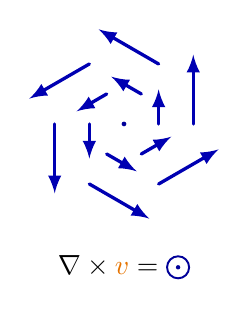
\begin{tikzpicture}
            \def\ang{60}
            \def\N{6}
            \fill[myblue] (0,0) circle (\r);
            \foreach \R in {0.44,0.88}{
                \foreach \i [evaluate={\ang=\i*360/\N;}] in {1,...,\N}{
                    \draw[vector] (\ang:\R) --++ (\ang+90:\R);
                }
            }
            \node at (0,-1.3*\R) {$\nabla \times {{\color{veccol}\boldsymbol{v}}} = \Cout$};
        \end{tikzpicture}
    \end{subfigure}
    \begin{subfigure}{.19\textwidth}
        \centering
        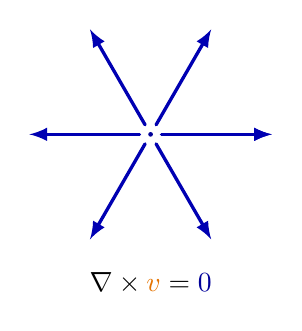
\begin{tikzpicture}
            \fill[myblue] (0,0) circle (\r);
            \foreach \i [evaluate={\ang=\i*360/\N;}] in {0,...,\N}{
                \draw[vector] (\ang:0.1*\R) --++ (\ang:\R);
            }
            \node at (0,-1.35*\R) {$\nabla \times {{\color{veccol}\boldsymbol{v}}} = \null$};
        \end{tikzpicture}
    \end{subfigure}
    \begin{subfigure}{.19\textwidth}
        \centering
        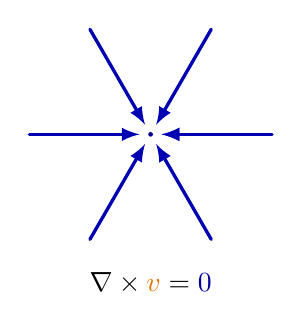
\begin{tikzpicture}
            \fill[myblue] (0,0) circle (\r);
            \foreach \i [evaluate={\ang=\i*360/\N;}] in {0,...,\N}{
                \draw[vector] (\ang:1.1*\R) -- (\ang:0.1*\R);
            }
            \node at (0,-1.35*\R) {$\nabla \times {{\color{veccol}\boldsymbol{v}}} = \null$};
        \end{tikzpicture}
    \end{subfigure}
    \begin{subfigure}{.19\textwidth}
        \centering
        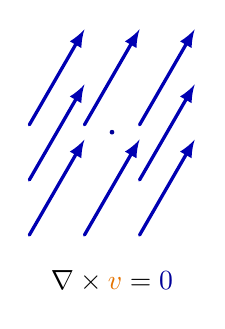
\begin{tikzpicture}
            \def\ang{60}
            \fill[myblue] (0,0) circle (\r);
            \foreach \x/\y in {-1/0,-1/1,0/1,1/1,1/0,-1/-1,0/-1,1/-1}{
                \draw[vector] (\x*0.5*\R,\y*0.5*\R) ++ (\ang-180:\R/2) --++ (\ang:\R);
            }
            \node at (0,-1.35*\R) {$\nabla \times {{\color{veccol}\boldsymbol{v}}} = \null$};
        \end{tikzpicture}
    \end{subfigure}
    \begin{subfigure}{.19\textwidth}
        \centering
        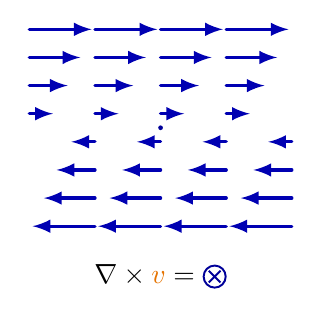
\begin{tikzpicture}
            \def\ang{60}
            \def\Ny{4}
            \def\Nx{4}
            \def\L{2.5}
            \fill[myblue] (0,0) circle (\r);
            \foreach \i [evaluate={\y=(\i-0.5)*(\L/2)/(\Ny-0.5); \r=0.3*\i^(0.7)}] in {1,...,\Ny}{
                \foreach \j [evaluate={\x=-\L/2+(\j-1.5)*\L/(\Nx-1);}] in {1,...,\Nx}{
                    \draw[vector] ( \x, \y) --++ ( \r,0);
                    \draw[vector] (-\x,-\y) --++ (-\r,0);
                }
            }
            \node at (0,-1.35*\R) {$\nabla \times {{\color{veccol}\boldsymbol{v}}} = \Cin$};
        \end{tikzpicture}
    \end{subfigure}
    \caption{Curl of vector fields}
    \label{fig:curl-examples}
\end{figure}

\subsection{Line Integrals}

\footnote{\href{https://trello.com/c/byu9Pyy8}{Calculus with Analytic Geometry by George F. Simmons, 2nd}, p. 751}
Throughout our discussion we assime that the functions under discussion have all the continuity and differentiability
properties that are needed in any given situation

If a charge is moving in an electromagnetic field with a constant force $\boldsymbol{F}$ (constant in both direction and
magnitude), then we know that the work done by this force is the product of the component of $\boldsymbol{F}$ in the
direction of motion and the distance the charged particle moves, i.e.

\begin{equation}
    W = \boldsymbol{F} \cdot \Delta \boldsymbol{R}
\end{equation}

where $\boldsymbol{R}$ is the vector from the initial position of the particle to its final position. Now suppose that
$\boldsymbol{F}$ is not constant, but instead is a vector function that varies from point to pint throughout a certain
region of the plane, say

\begin{equation}\label{eq:vector-valued-function}
    \boldsymbol{F} = \boldsymbol{F}(x, y) = M(x, y)\boldsymbol{\hat{i}} + N(x, y)\boldsymbol{\hat{j}}
\end{equation}

\begin{tcolorbox}[
    enhanced,
    arc=3mm,boxrule=1.5mm,
    frame hidden,colback=blue!10!white,
    borderline={1mm}{0mm}{blue,dotted}
]
    \phantomsection\hypertarget{vector-field}
    The vector-value function~\ref{eq:vector-valued-function} is usually called \textit{force field}. More generally,
    a \textit{vector field} in the plane is any vector-valued function that associates a vector with each point $(x, y)$
    in a certain plane region $R$. In this context a function whose values are numbers (scalars) is called a
    \textit{scalar field}. Every scalar field $f(x, y)$ gives rise to a corresponding vector field

    \begin{equation}
        \nabla f(x, y) = \frac{\partial f}{\partial x}\boldsymbol{\hat{i}} + \frac{\partial f}{\partial y}\boldsymbol{\hat{y}}
    \end{equation}

    This is called the \textit{gradient field} of $f$. Some vector fields are gradient fields, but most are not. Those
    gradient fields, however, are of special importance
\end{tcolorbox}

Suppose also that this variable force pushes the charged particle along a smooth curve $C$ with a parametric equations

\begin{equation}
    x = x(t) \text{\ \ \ \ \ \ and \ \ \ \ \ \ } y = y(t)\text{, \ \ \ \ \ \ } t_1 \le t \le t^2
\end{equation}

The work done by this force is denoted by

\begin{equation}
    \int_{C} \boldsymbol{F} \cdot d\boldsymbol{R} \text{\ \ \ \ \ \ or \ \ \ \ \ \ } \int_{C}M(x, y)dx + N(x, y)dy
\end{equation}


\includegraphics[width=0.05\textwidth]{可莉-86.png} This is called the \textbf{line integral}

We approximate the curve by a polygonal path as shown in Fig.~\ref{fig:line-integral}. That is, choose points
$P_0 = A, P_1, P_2, \ldots, P_{n - 1}, P_n = B$ along C in this order; let $\boldsymbol{R_k}$ be the position vector of
$P_k$ and define the $n$ incremental vectors by $\Delta \boldsymbol{R_k} = \boldsymbol{R_{k + 1}} - \boldsymbol{R_k}$,
where $k = 0, 1, \ldots, n - 1$

\begin{figure}[H]
    \centering
    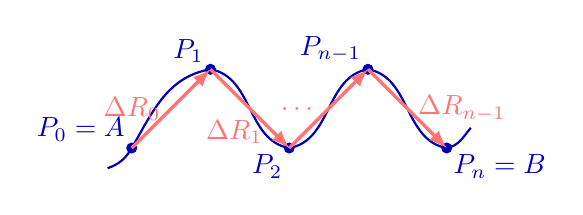
\begin{tikzpicture}
        \colorlet{xcol}{blue!70!black}
        \colorlet{acol}{red!50!blue!80!black!80}
        \tikzstyle{vector}=[->,very thick,xcol,line cap=round]

        \def\ul{0.6}
        \def\Ra{1.4}
        \def\Rb{0.8}
        \coordinate (A) at (0, 0);
        \coordinate (B) at (1,1);
        \coordinate (C) at (2,0);
        \coordinate (D) at (3,1);
        \coordinate (E) at (4,0);

        \draw[xcol,thick]
        (A)++(-140:0.4) to[out=20,in=-120]
        (A) to[out=60, in=-170]
        (B) to[out=-10, in=170]
        (C) to[out=10, in=-170]
        (D) to[out=-10, in=170,]
        (E) to[out=10, in=-130]++ (40:0.4);

        \fill[xcol] (A) circle (2pt) node[above left=-1] {$P_0 = A$};
        \fill[xcol] (B) circle (2pt) node[above left=-1] {$P_1$};
        \fill[xcol] (C) circle (2pt) node[below left=-1] {$P_2$};
        \fill[xcol] (D) circle (2pt) node[above left=-1] {$P_{n - 1}$};
        \fill[xcol] (E) circle (2pt) node[below right=-1] {$P_n = B$};

        \draw [very thick, -{latex[scale=3.0]}, white!45!red] (A) -- (B)node[pos=0.5,left]{$\Delta\boldsymbol{R_0}$};
        \draw [very thick, -{latex[scale=3.0]}, white!45!red] (B) -- (C)node[pos=0.8,left]{$\Delta\boldsymbol{R_1}$};
        \draw [very thick, -{latex[scale=3.0]}, white!45!red] (C) -- (D)node[pos=0.5,left]{\ldots};
        \draw [very thick, -{latex[scale=3.0]}, white!45!red] (D) -- (E)node[pos=0.5,right]{$\Delta\boldsymbol{R_{n - 1}}$};
    \end{tikzpicture}
    \caption{Approximating line integral}
    \label{fig:line-integral}
\end{figure}

If we denote by $\boldsymbol{F_k}$ the value of the vector function $\boldsymbol{F}$ at $P_k$ and form the sum

\begin{equation}
    \sum_{k = 0}^{n - 1}\boldsymbol{F_k} \cdot \Delta\boldsymbol{R_k}
\end{equation}

then the \textit{line integral of} $\boldsymbol{F}$ \textit{along} $C$ is defined to be the limit of sums

\begin{equation}
    \int_{C} \boldsymbol{F} \cdot d\boldsymbol{R} = \lim \sum_{k = 0}^{n - 1}\boldsymbol{F_k} \cdot \Delta\boldsymbol{R_k}
\end{equation}

\begin{tcolorbox}[enhanced,arc=3mm,boxrule=1.5mm,
    frame hidden,colback=blue!10!white,
    borderline={1mm}{0mm}{blue,dotted}
]
    \footnote{\href{https://trello.com/c/byu9Pyy8}{Calculus with Analytic Geometry by George F. Simmons, 2nd}, p. 757} It
    will often be necessary to consider situations in which th path of integration $C$ is a \textit{closed} curve. In this
    case a line integral is usually written with a small circle on the integral sign, as in

    \[
        \oint_{C} \boldsymbol{F} \cdot d\boldsymbol{R}
    \]
\end{tcolorbox}

\subsubsection{The Fundamental Theorem of Calculus}

\footnote{\href{https://trello.com/c/byu9Pyy8}{Calculus with Analytic Geometry by George F. Simmons, 2nd}, p. 206}We
intuitively know that the \textbf{definite integral} of a continuous function is the limit of approximating sums, i.e.

\begin{equation}\label{eq:riemann-integral}
    \int_{a}^{b} f(x)dx = \lim\limits_{\text{max}\Delta x_k \rightarrow 0}\sum_{k = 1}^{n} f(x_k^*)\Delta x_k
\end{equation}

The definite integral which is defined here is often called the \textbf{Riemann integral}, in honor of the 19th-centry
German mathematician who was the first to give a careful discussion of integrals of discontinuous
functions\footnote{\href{https://trello.com/c/byu9Pyy8}{Calculus with Analytic Geometry by George F. Simmons, 2nd}, p. 202}

Eq.~\ref{eq:riemann-integral} immediately proves the following properties of definite integral\footnote{\href{https://trello.com/c/byu9Pyy8}{Calculus with Analytic Geometry by George F. Simmons, 2nd}, p. 214}:

\begin{equation}\label{eq:definite-integral-reverse}
    \int_a^b f(x)dx = -\int_b^a f(x)dx
\end{equation}

\begin{equation}
    \int_a^b cf(x)dx = c\int_a^b f(x)dx
\end{equation}

\begin{equation}
    \int_a^b [f(x) + g(x)]dx = \int_a^b f(x)dx + \int_a^b g(x)dx
\end{equation}

\begin{equation}
    \text{if } f(x) \le g(x) \text{ on } [a, b] \text{,} \text{\ \ \ \ \ \ then \ \ \ \ \ \ }  \int_a^b f(x)dx \le \int_a^b g(x)dx
\end{equation}

\begin{equation}\label{eq:definite-integral-additive}
    \int_a^b f(x)dx = \int_a^c f(x)dx + \int_c^b f(x)dx
\end{equation}



This definition works for integrals of rather \textit{simple} functions such as

\[
    \int_0^b xdx = \frac{b^2}{2}
\]

but not for such complicate integrals as

\[
    \int_{0}^{1}\frac{x^4}{(7 + x^5)^{\frac{1}{3}}} dx
\]

The Fundamental Theorem of Calculus links the concept of differentiating a function with the concept of integrating a
function, showing that \roundinlinebox[green]{these two operations are essentially inverse of one another}. Before
the discover of this theorem, however, it was not recognized that these two operations were related. Ancient Greek
mathematicians knew how to compute area via infinitesimals, an operation that we would now call integration. The origins
of differentiation likewise predate the fundamental theorem of calculus by hundreds of years. \textbf{The
historical relevance of the fundamental theorem of calculus is not the ability to calculate these operations, but the
realization that the two seeminly distinct operations are actually closely related}

\begin{Theorem}{\href{https://en.wikipedia.org/wiki/Fundamental\_theorem\_of\_calculus\#First\_part}{The First Fundamental Theorem of Calculus}}{fundamental-theorem-of-calculus-part-1}
    Let $f$ be a continuous real-valued function defined ona closed interval $[a, b]$. Let $F$ be the function defined,
    for all $x$ in $[a, b]$, by

    \begin{equation}
        F(x) = \int_a^x f(t) dt
    \end{equation}

    Then $F$ is uniformly continuous on $[a, b]$ and differentiable on the open interval $(a, b)$ and

    \begin{equation}
        F'(x) = f(x)
    \end{equation}

    for all $x$ in $(a, b)$ so $F$ is an antiderivative of $f$
\end{Theorem}

\paragraph{Proof of Theorem~\ref{theo:fundamental-theorem-of-calculus-part-1}}

\footnote{\href{https://en.wikipedia.org/wiki/Fundamental_theorem_of_calculus\#Proof\_of\_the\_first\_part}{Proof of the first part, Fundamental theorem of calculus}, Wikipedia}
For a given function $f$, define the function $F(x)$ as

\[
    F(x) = \int_a^x f(t) dt
\]

For any two number $x_1$ and $x_1 + \Delta x$ in $[a, b]$, we have

\begin{align}
    F(x_1 + \Delta x) - F(x_1) &= \int_a^{x_1 + \Delta x} f(t) dt - \int_a^{x_1} f(t) dt \\
    &= \int_a^{x_1 + \Delta x} f(t) dt + \int_{x_1}^a f(t) dt \text{ (by Eq.~\ref{eq:definite-integral-reverse})}\\
    &= \int_{x_1}^{x_1 + \Delta x} f(t)dt\label{eq:F-del-x-minus-F} \text{ (by Eq.~\ref{eq:definite-integral-additive})}
\end{align}

To be able to go any further, we shall introduce the \textit{Mean value theorem for definite integrals}

\begin{Theorem}{\href{https://en.wikipedia.org/wiki/Mean\_value\_theorem\#First\_mean\_value\_theorem\_for\_definite\_integrals}{Mean Value Theorem for Definite Integrals}}{mean-value-theorem-def-integrals}
    If $f: [a, b] \rightarrow \mathbb{R}$ is continuous and $g$ is an integrable function that does not change sign on
    $[a, b]$, then there exists $c$ in $(a, b)$ such that

    \begin{equation}
        \int_a^b f(x)g(x)dx = f(c)\int_a^b g(x)dx
    \end{equation}

    \tcblower

    \paragraph{Proof}

    suppose $f: [a, b] \rightarrow \mathbb{R}$ is continuous and $g$ is a \textit{non-negative} integrable function
    on $[a, b]$. By the \href{https://en.wikipedia.org/wiki/Extreme\_value\_theorem}{extreme value theorem}, there
    exists $m$ and $M$ such that for each $x$ in $[a, b]$, $m \le f(x) \le M$ and $f[a, b] = [m, M]$. Since $g$ is
    \textit{non-negative},

    \begin{equation}
        m\int_a^b g(x)dx \le \int_a^b f(x)g(x)dx \le M\int_a^b g(x)dx
    \end{equation}

    If $g(x) = 0$,

    \begin{equation}
        0 \le \int_a^b f(x)g(x)dx \le 0
    \end{equation}

    \begin{equation}
        \int_a^b f(x)g(x)dx = 0
    \end{equation}

    so for any $c \in [a, b]$

    \begin{equation}
        \int_a^b f(x)g(x)dx = f(c)\int_a^b g(x)dx = 0
    \end{equation}

    If $g(x) \ne 0$,

    \begin{equation}
        m \le \frac{1}{\int_a^b g(x)dx}\int_a^b f(x)g(x)dx \le M
    \end{equation}

    By the \href{https://en.wikipedia.org/wiki/Intermediate\_value\_theorem}{intermediate value theorem}, $f$ attains
    very value of the interval $[m, M]$ so for some $c$ in $[a, b]$:

    \begin{equation}
        f(c) = \frac{1}{\int_a^b g(x)dx}\int_a^b f(x)g(x)dx
    \end{equation}

    that is,

    \begin{equation}
        f(c)\int_a^b g(x)dx = \int_a^b f(x)g(x)dx
    \end{equation}

    Finally, if $g$ is negative on $[a, b]$, we can still get the same result.

    \begin{flushright}
        
\includegraphics[width=0.05\textwidth]{胡桃-28.png}
    \end{flushright}
\end{Theorem}

By having $g(x) = 1$ in \hyperref[theo:mean-value-theorem-def-integrals]{mean value theorem for integration}, we have

\begin{equation}
    \int_a^b f(x)dx = f(c)(b - a)
\end{equation}

We can now move on with Eq.~\ref{eq:F-del-x-minus-F}. There exists a real number $c \in [x_1, x_1 + \Delta x]$ such that

\begin{equation}
    F(x_1 + \Delta x) - F(x_1) = \int_{x_1}^{x_1 + \Delta x} f(t)dt = f(c)\Delta x
\end{equation}

so

\begin{equation}
    \frac{F(x_1 + \Delta x) - F(x_1)}{\Delta x} = f(c)
\end{equation}

\begin{equation}
    \lim\limits_{\Delta x \rightarrow 0}\frac{F(x_1 + \Delta x) - F(x_1)}{\Delta x} = \lim\limits_{\Delta x \rightarrow 0} f(c)
\end{equation}

that is,

\begin{equation}
    F'(x_1) = f(x_1)
\end{equation}

\begin{Corollary}{\href{https://en.wikipedia.org/wiki/Fundamental\_theorem\_of\_calculus\#Corollary}{Corollary} of Theorem~\ref{theo:fundamental-theorem-of-calculus-part-1}}{fundamental-theorem-of-calculus-part-1-corollary}
    If $f$ is a real-valued continuous function on $[a, b]$ and $F$ an antiderivative of $f$ in $[a, b]$, then

    \begin{equation}
        \int_a^b f(t)dt = F(b) - F(a)
    \end{equation}

    Note that the corollary assumes continuity on the whole interval. This result is strenghened slightly in
    Theorem~\ref{theo:fundamental-theorem-of-calculus-part-2}
\end{Corollary}

\paragraph{Proof of Corollary~\ref{cor:fundamental-theorem-of-calculus-part-1-corollary}}\footnote{}

\footnote{\href{https://en.wikipedia.org/wiki/Fundamental\_theorem\_of\_calculus\#Proof\_of\_the\_corollary}{Proof of the corollary, Fundamental theorem of calculus}, Wikipedia}
Suppose $F$ is an antiderivative of $f$, which is continuous on $[a, b]$. Let $G(x)$ also be an antiderivative of $f$:

\begin{equation}
    G(x) = \int_a^x f(t)dt
\end{equation}

By Theorem~\ref{theo:mean-value-theorem-def-integrals}, we have

\begin{align}
    F'(x) = f(x) \\
    G'(x) = f(x)
\end{align}

It is easy to see then

\begin{equation}
    F - G = c
\end{equation}

where $c$ is a constant. That is, there is a number $c$ such that

\begin{equation}
    G(x) = F(x) + c
\end{equation}

for all $x \in [a, b]$

Let $x = a$, we have

\begin{equation}
    F(a) + c = G(a) = \int_a^a f(t)dt = 0
\end{equation}

which means

\begin{equation}
    c = - F(a)
\end{equation}

or

\begin{equation}
    G(x) = F(x) - F(a)
\end{equation}

Therefore

\begin{equation}
    \int_a^b f(t) dt = G(b) = F(b) - F(a)
\end{equation}

\begin{figure}[H]
    \begin{flushright}
        
\includegraphics[width=0.05\textwidth]{胡桃-28.png}
    \end{flushright}
\end{figure}

\begin{Theorem}{\href{https://en.wikipedia.org/wiki/Fundamental\_theorem\_of\_calculus\#Second\_part}{The Second Fundamental Theorem of Calculus}: Newton-Leibniz Theorem\phantomsection\hypertarget{fundamental-theorem-of-calculus-part-2}}{fundamental-theorem-of-calculus-part-2}
    Let $f$ be a real-valued function on a closed interval $[a, b]$ and $F$ a continuous function on $[a, b]$ which is
    an antiderivative of $f$ in $(a, b)$:

    \begin{equation}
        F'(x) = f(x)
    \end{equation}

    If $f$ is \hyperref[eq:riemann-integral]{Riemann integrable} on $[a, b]$, then

    \begin{equation}
        \int_a^b f(x)dx = F(b) - F(a)
    \end{equation}

    Here we \textbf{do not assume $f$ is continuous}
\end{Theorem}

\paragraph{Proof of Theorem~\ref{theo:fundamental-theorem-of-calculus-part-2}}

\footnote{\href{https://en.wikipedia.org/wiki/Fundamental\_theorem\_of\_calculus\#Proof\_of\_the\_second\_part}{Proof of the second part, Fundamental theorem of calculus}, Wikipedia}
Let $f$ be \hyperref[eq:riemann-integral]{Riemann integrable} on $[a, b]$ and let $f$ admit an antiderivative $F$ on
$(a, b)$ such that $F$ is continuous on $[a, b]$.

Begin with the quantity $F(b) - F(a)$. Let there be numbers $x_0, \ldots, x_n$ such that

\begin{equation}
    a = x_0 < x_1 < x_2 < \ldots < x_{n - 1} < x_n = b
\end{equation}

If follows that

\begin{equation}
    F(b) - F(a) = F(x_n) - F(x_0)
\end{equation}

Now, we add each $F(x_i)$ along with its additive inverse, so that the resulting quantity is equal:

\begin{align}
    &F(b) - F(a) \\
    ={}& F(x_n) + [-F(x_{n - 1} + F(x_{n - 1})] + \ldots + [-F(x_{1} + F(x_{1})] - F(x_0) \\
    ={}& [F(x_n) - F(x_{n - 1})] + [F(x_{n - 1}) - F(x_{n - 2})] + \ldots + [F(x_2) - F(x_1)] + [F(x_{1}) - F(x_0)] \\
    ={}& \sum_{i = 1}^n \left[ F(x_i) - F(x_{i - 1}) \right] \label{eq:sum-of-subtractives}
\end{align}

Since $F$ is differentiable on interval $(a, b)$ and continuous on $[a, b]$, it is also differentiable on each interval
$(x_{i - 1}, x_i)$ and continuous on each interval $[x_{i - 1}, x_i]$. According to the
\hyperlink{theo:mean-value-theorem}{Mean Value Theorem}, for each $i$ there exists a $c_i$ in $(x_{i - 1}, x_i)$ such
that

\begin{equation}
    F(x_i) - F(x_{i - 1}) = F'(c_i)(x_i - x_{i - 1})
\end{equation}

Plugging this equation into Eq.~\ref{eq:sum-of-subtractives}, we get

\begin{equation}
    F(b) - F(a) = \sum_{i = 1}^n \left[ F'(c_i)(x_i - x_{i - 1}) \right] = \sum_{i = 1}^n \left[ f(c_i)\Delta x_i \right]
\end{equation}

We are describing the area of a rectangle, with the width times the height, and we are adding the areas together. Each
rectangle, by virtue of the Mean Value Theorem, describes an approximation of the curve section it is drawn over. Also
$\Delta x_i$ need not be the same for all values of $i$. What we will do is to approximate the curve with $n$
rectangles. As the widths of the partitions get smaller and $n$ increases, we get closer to the actual areas

Since $f$ is Riemann integrable:

\begin{equation}
    \lim\limits_{\Vert \Delta x_i \Vert \rightarrow 0}F(b) - F(a) = \lim\limits_{\Vert \Delta x_i \Vert \rightarrow 0}\sum_{i = 1}^n \left[ f(c_i)\Delta x_i \right]
\end{equation}

\begin{equation}
    F(b) - F(a) = \lim\limits_{\Vert \Delta x_i \Vert \rightarrow 0}\sum_{i = 1}^n \left[ f(c_i)\Delta x_i \right]
\end{equation}

\begin{equation}
    F(b) - F(a) = \int_a^b f(x) dx
\end{equation}

\begin{figure}[H]
    \begin{flushright}
        
\includegraphics[width=0.05\textwidth]{胡桃-28.png}
    \end{flushright}
\end{figure}

\subsubsection{Independence of Path \& Conservative Fields}

\footnote{\href{https://trello.com/c/byu9Pyy8}{Calculus with Analytic Geometry by George F. Simmons, 2nd}, p. 758} \hyperlink{vector-field}{We have already known that the vector field is the gradient of a scalar field}. The
\hyperlink{fundamental-theorem-of-calculus-part-2}{Fundamental Theorem of Calculus of single-variable} in the case of
2 variables can be derived as follows:

\begin{align}
    \int_C\boldsymbol{F}\cdot d\boldsymbol{R} &= \int_C \nabla f \cdot d\boldsymbol{R} \\
    &= \int_a^b\left( \nabla f \cdot \frac{d\boldsymbol{R}}{dt} \right)dt \\
    &= \int_a^b\left[ \left( \frac{\partial f}{\partial x}\boldsymbol{\hat{x}} + \frac{\partial f}{\partial y}\boldsymbol{\hat{y}} \right)  \cdot \frac{d(x\boldsymbol{\hat{x}} + y\boldsymbol{\hat{y}})}{dt} \right]dt \\
    &= \int_a^b\left( \frac{\partial f}{\partial x}\frac{\partial x}{\partial t} + \frac{\partial f}{\partial y}\frac{\partial y}{\partial t} \right)dt \\
    &= \int_a^b \frac{d}{dt}f(x, y)dt \\
    &= f(b) - f(a)
\end{align}

\begin{Theorem}{Fundamental Theorem of Calculus for Line Integrals}{fundamental-theorem-of-calculus-for-line-integrals}
    If a vector field $\boldsymbol{F}$ is the gradient of some scalar field $f$ in a region $R$, so that
    $\boldsymbol{F} = \nabla f$ in $R$, and if $C$ is any piecewise smooth curve in $R$ with initial and final points
    $A$ and $B$, then

    \begin{equation}\label{eq:fundamental-theorem-of-calculus-for-line-integrals}
        \int_C\boldsymbol{F} \cdot d\boldsymbol{R} = f(B) - f(A)
    \end{equation}
\end{Theorem}

The right side of the Eq.~\ref{eq:fundamental-theorem-of-calculus-for-line-integrals} depends only on the points $A$ and
$B$ and not at all on the path $C$ that joins them. The line integral on the left side of
Eq.~\ref{eq:fundamental-theorem-of-calculus-for-line-integrals} therefore has the same value for all paths $C$ from $A$
to $B$. This can be expressed by saying that the \highlight[green]{line integral of a gradient field is independent
of the path} 
\includegraphics[width=0.05\textwidth]{心海-17.png}. Next, it is clear from
Eq.~\ref{eq:fundamental-theorem-of-calculus-for-line-integrals} that \highlight[green]{if $C$ is a closed path, then} 
\includegraphics[width=0.05\textwidth]{心海-18.png}

\begin{equation}\label{eq:closed-path-line-int}
    \oint_C\boldsymbol{F} \cdot d\boldsymbol{R} = 0
\end{equation}

These argument show that

\begin{figure}[H]
    \newtcbox{\inlineframe}[1][green]{
        on line,
        arc=5pt,
        colback=white,
        colframe=#1!50!white,
        before upper={\rule[-3pt]{0pt}{10pt}},
        boxrule=1pt,
        boxsep=0pt,left=6pt,right=6pt,top=2pt,bottom=2pt
    }

    \centering
    \begin{tikzpicture}
        \matrix (m) [matrix of math nodes,row sep=0.8em,column sep=3em,minimum width=2em] {
            \quad & \text{\inlineframe{\hyperref[theo:fundamental-theorem-of-calculus-for-line-integrals]{Integral is independent of path}}} \\
            \text{\inlineframe{\hyperlink{vector-field}{Gradient field}}} & \quad \\
            \quad & \text{\inlineframe{\hyperref[eq:closed-path-line-int]{Integral around closed path is zero}}} \\};
        \path[-stealth]
        (m-2-1) edge [double] node [above] {} (m-1-2)
        (m-2-1) edge [double] node [below] {} (m-3-2);
    \end{tikzpicture}\qquad

    \caption{The symbol $\Rightarrow$ means ``implies"}
    \label{fig:gradient-field}
\end{figure}

We are going to show that these 3 properties are equivalent, in the sense that each implies the other two.

Suppose that the line integral of the vector field $\boldsymbol{F}$ is independent of the path. We shall approve that
the line integral of the vector field $\boldsymbol{F}$ around a closed path is zero.

We examine the figure below, in which two points $A$ and $B$ are chosen on the closed path $C$. These points divide $C$
into paths $C_1$, from $A$ to $B$, and $C_2$, from $B$ to $A$.

\begin{figure}[H]
    \centering
    \begin{tikzpicture}
        \coordinate  (A) at (-1.8,-.2);
        \coordinate  (B) at (2.42,-.45);
        \coordinate  (C) at (-.3,1);
        \coordinate  (D) at (1.8,-1.18);

        \draw[red,use Hobby shortcut,closed=true]
        (-1.8,-.2) .. (-1.6,.5) .. (-1,.9) ..
        (-.3,1) .. (1,.7) .. (2,.2) .. (2.22,0) ..
        (2.42,-.45) .. (2.25,-1) ..
        (1.8,-1.18) .. (1.2,-1) ..
        (0,-.8) ..
        (-.9,-.9) .. (-1.5,-.7)
        ;

        \fill[black] (A) circle (2pt) node[left] {A};
        \fill[black] (B) circle (2pt) node[right] {B};

        \fill[black] (C) circle (0pt) node[above] {$C_1 \rightarrow$};
        \fill[black] (D) circle (0pt) node[below] {$\leftarrow C_2$};
    \end{tikzpicture}
\end{figure}

Since both $C_1$ and $-C_2$ are paths from $A$ to $B$,
the assumption of independence of path implies that

\begin{equation}
    \int_{C_1}\boldsymbol{F}\cdot d\boldsymbol{R} = \underbrace{\int_{-C_2}\boldsymbol{F}\cdot d\boldsymbol{R} = -\int_{C_2}\boldsymbol{F}\cdot d\boldsymbol{R}}_{Eq.~\ref{eq:definite-integral-reverse}}
\end{equation}

It them follows that

\begin{equation}
    \int_{C_1}\boldsymbol{F}\cdot d\boldsymbol{R} + \int_{C_2}\boldsymbol{F}\cdot d\boldsymbol{R} = \oint_C\boldsymbol{F}\cdot d\boldsymbol{R} = 0
\end{equation}

\begin{figure}[H]
    \begin{flushright}
        
\includegraphics[width=0.05\textwidth]{胡桃-28.png}
    \end{flushright}
\end{figure}

Then we can easily reverse this argument to show that the integral from $A$ to $B$ is independent of the path

\begin{figure}[H]
    \newtcbox{\inlineframe}[1][green]{
        on line,
        arc=5pt,
        colback=white,
        colframe=#1!50!white,
        before upper={\rule[-3pt]{0pt}{10pt}},
        boxrule=1pt,
        boxsep=0pt,left=6pt,right=6pt,top=2pt,bottom=2pt
    }

    \centering
    \begin{tikzpicture}
        \matrix (m) [matrix of math nodes,row sep=0.8em,column sep=3em,minimum width=2em] {
            \quad & \text{\inlineframe{\hyperref[theo:fundamental-theorem-of-calculus-for-line-integrals]{Integral is independent of path}}} \\
            \text{\inlineframe{\hyperlink{vector-field}{Gradient field}}} & \quad \\
            \quad & \text{\inlineframe{\hyperref[eq:closed-path-line-int]{Integral around closed path is zero}}} \\};
        \path[-stealth]
        (m-2-1) edge [double] node [above] {} (m-1-2)
        (m-2-1) edge [double] node [below] {} (m-3-2);

        \path[stealth-stealth]
        (m-1-2) edge [double] node [below] {} (m-3-2);
    \end{tikzpicture}\qquad

    \caption{The updated Fig.~\ref{fig:gradient-field}}
    \label{fig:closed-line-integral}
\end{figure}

To complete the proof of the equivalence of the 3 properties, it suffices to show that if $\boldsymbol{F}$ is a vector
fioeld whose line integral is independent of path, then $\boldsymbol{F} = \nabla f$ for some scalar field $f$.

\begin{figure}[H]
    \centering
    \begin{tikzpicture}[
    x=1bp,
        y=-1bp,
        use Hobby shortcut,
        every circle/.style={radius=2},
        thick,
        my marks/.style={},
        arrow mark/.style={
          /my marks/.append style={
            mark=at position #1 with {\arrow[ultra thick]{stealth}},
          },
        },
        reversed arrow mark/.style={
          /my marks/.append style={
            mark=at position #1 with {\arrowreversed[ultra thick]{stealth}},
          },
        },
        do marks/.style={
          decorate,
          postaction={
            decoration={
              markings,
              /my marks,
            },
            decorate,
          },
        },
    ]
    \fill (60,57) circle;
    \draw[
      arrow mark=.14,
      do marks,
    ]
      (34,56)..(53,44)..(64,45)..(73,57)..(60,68)..(49,61)..(54,53)
    ;
    \draw[
      arrow mark=1,
      do marks,
      shorten >=1pt,
    ]
      (134,83)..(117,75)..(86,91)..(51,103)..(1,58)..(53,12)..(87,18)..
      (113,25)..(148,0)
    ;
    \fill (118,50) coordinate (cross) circle;
    \draw[
      arrow mark=.06,
      reversed arrow mark=.24,
      reversed arrow mark=.78,
      arrow mark=.92,
      do marks,
    ]
      (152,86)..(cross)..(59,26)..(21,56)..(55,84)..(cross)..(152,11)
    ;
    \node[
      below left,
      inner sep=0pt,
      outer sep=0pt,
      font=\sffamily,
    ] at (current bounding box.south east) {HL};
  \end{tikzpicture}
\end{figure}